% REVISÃO BIBLIOGRÁFICA------------------------------------------------------------------

\chapter{REVISÃO DE LITERATURA}
\label{chap:revisao_bibliografica}
\section{Objetivos de desenvolvimento sustentável}

Os países membros da Organização das Nações Unidas (ONU), em 2015, estabeleceram uma agenda de desenvolvimento sustentável para os próximos 15 anos, na qual se comprometeram a trabalhar para atingirem 17 Objetivos de Desenvolvimento Sustentável (ODS).
“Os ODS buscam assegurar os direitos humanos, acabar com a pobreza, lutar contra a desigualdade e a injustiça, alcançar a igualdade de gênero e o empoderamento de mulheres e meninas, agir contra as mudanças climáticas, bem como enfrentar outros dos maiores desafios de nossos tempos” \cite{pactoglobal}.

Atualmente, petróleo bruto, carvão e gás, que são fosseis e não renováveis, ainda são dominantes na produção de combustíveis. A utilização dos combustíveis fosseis gera diversos impactos ambientais não desejáveis como: a poluição do ar e o aquecimento global \cite{Gebremariam2018}.

O petróleo, descoberto em 1859, foi a fonte de energia mais importante do  XX. Segundo  a Organização das Exportações de Petróleo Países, OPEP, a demanda mundial de óleo combustível atingirá até 109,4 milhões de barris por dia, em 2040, dos quais 5,7 milhões de barris por dia serão destinados a demanda de óleo diesel.

Dos 17 Objetivos de Desenvolvimento Sustentável três tem relação direta com a diminuição do consumo de combustíveis derivados de petróleo: o objetivo 7 - energia acessível e energia acessível e limpa; o objetivo 12 – consumo e produção responsáveis e o objetivo 13 – ação contra a mudança global do clima \cite{ONU}.

O biodiesel surge como uma das alternativas, ambientalmente vantajosas, que poderiam ser utilizadas para redução do consumo  dos combustíveis fosseis como fonte de energia . 

\section{Álcoois e Ácidos  carboxílicos}

Os ácidos carboxílicos com cadeia carbônica  entre 4 e 22 carbonos, e os  álcoois entre 6 e 22 carbonos, são denominados graxos. Ambos são encontrados em plantas, nas quais estão diretamente ligados.
    
Os álcoois graxos são, industrialmente, interessantes por terem a capacidade de formar micelas, são tensoativos não iônicos, ou seja, surfactantes. A indústria de cosméticos tem interesse por  moléculas que apresentam características hidrofóbicas e uma extremidade polar, o que permite a formação de emulsões. Outras aplicações possíveis são  a produção de lubrificantes,  polímeros, para o aumento de viscosidade em óleos,  em fragrância e flavorizantes. Nos alimentos eles possibilitam uma variedade de texturas. Nos  fármacos desempenha um papel importante nas propriedades  ponto de fusão e solubilidade, caracterizadas pelo equilíbrio de fase sólido-líquido. \cite{Barbosa2012}
    
Os ácidos graxos tem  aplicações nas indústrias de  biodiesel, de cosméticos, de alimentos, entre outras, dentre essas aplicações destaca-se  a fabricação de biodiesel. 

O biodiesel é um combustível  derivado de óleos vegetais, gorduras animais e óleos de algas. A substituição do diesel pelo biodiesel é ambientalmente benéfica, visto que, ele é biodegradável,  sua queima emite menos gases poluentes e  partículas \cite{Hanna1999,Atadashi2011}.   Para o biodiesel de origem vegetal  o CO$_2$  absorvido durante o crescimento da  planta,   é liberado durante a sua queima, estabelecendo um ciclo fechado de carbono. O uso do biodiesel reduz em até  78\% as emissões líquidas de CO$_2$ \cite{Aparecida2006}. 
    
O biodiesel é produzido por meio da transesterificação,  reação na qual  os triglicerídeos reagem com álcoois, na presença de um catalisador, para produzir esteres de  ácido graxo e glicerina, essa produzida como subproduto \cite{Hoekman2012}.
    
Ainda referente à produção, O  biodiesel pode ser produzido da maioria dos triglicerídeos, centenas de matérias-primas são descritas na literatura. No entanto, as mais  utilizadas são o óleo de soja nos Estados Unidos, óleo de colza na Europa, óleo de palma no sudeste Ásia e o Brasil, produz  variadas matérias-primas para a produção de biodiesel,  como a soja, o girassol, a mamona, o milho, o pinhão manso, o caroço de algodão, a canola, o babaçu, o buriti, o dendê, a macaúba e o amendoim, além das de origem animal como o sebo bovino e as gorduras de frango e de suínos, sendo o mais utilizado o biodiesel de soja \cite{Ramos2017,Hoekman2012}.
    
Os ácidos carboxílicos mais presentes nos biodieseis são mostrados na Tabela \ref{tab:Grupo} dieseis  derivados  de óleos vegetais e gorduras animais: ácido palmítico, ácido esteárico , ácido oleico, ácido linoléico e ácido linolênico. \cite{Hoekman2012,Ramos2017}.
    
\begin{table}[H]
    \centering
    \caption{Grupos de ácidos graxos típicos em biodiesel}
    \begin{tabular}{lccc}
    \hline
    Nome & N$^0$ CAS  & Fórmula Molecular  & Estrutura Molecular  \\
    \hline
    Ácido Láurico & 143-07-7 & \ch{C12H24O2} & \raisebox{-0.5\height}{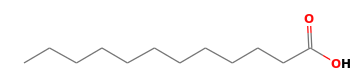
\includegraphics[width=0.4\linewidth]{dados/figuras/Ac_laurico.png}} \\
    Ácido Miristico & 544-63-8 & \ch{C14H28O2} & \raisebox{-0.5\height}{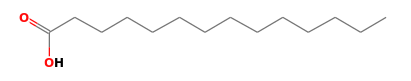
\includegraphics[width=0.4\linewidth]{dados/figuras/Ac_miristico.png}} \\
    Ácido Miristoléico & 544-63-9 & \ch{C14H28O2} & \raisebox{-0.5\height}{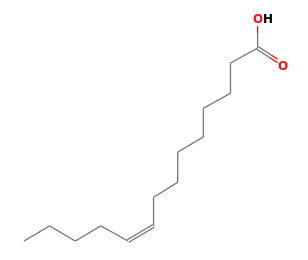
\includegraphics[width=0.25\linewidth]{dados/figuras/Ac_myristoleic.png}} \\
    Ácido Palmítico & 57-10-3 & \ch{C16H32O2} & \raisebox{-0.5\height}{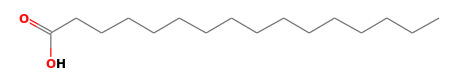
\includegraphics[width=0.4\linewidth]{dados/figuras/Ac_palmitico.png}} \\
    
    \end{tabular}
    \label{tab:Grupo}
\end{table}

\begin{table}[H]
    \centering
    \begin{tabular}{lccc}
    Ácido Palmitoléico & 373-49-9 & \ch{C16H32O2} & \raisebox{-0.5\height}{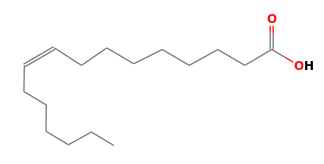
\includegraphics[width=0.3\linewidth]{dados/figuras/Ac_palmitoleico.png}} \\
    Ácido Esteárico & 57-11-4 & \ch{C18H36O2} & \raisebox{-0.5\height}{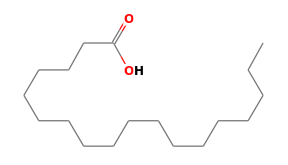
\includegraphics[width=0.4\linewidth]{dados/figuras/ac_estearico.png}} \\
    Ácido Oleico & 112-80-1 & \ch{C18H34O2} & \raisebox{-0.5\height}{\includegraphics[width=0.4\linewidth]{dados/figuras/Ac_oleico.png}} \\
    Ácido Linoleico & 60-33-3 & \ch{C18H32O2} & \raisebox{-0.5\height}{\includegraphics[width=0.4\linewidth]{dados/figuras/Ac_linoleico_1.png}} \\
    Ácido Linolênico & 463-40-1 & \ch{C18H30O2} & \raisebox{-0.5\height}{\includegraphics[width=0.4\linewidth]{dados/figuras/Ac_linolenico.png}} \\
    Ácido Araquídico & 506-30-9 & \ch{C20H40O2} & \raisebox{-0.5\height}{\includegraphics[width=0.4\linewidth]{dados/figuras/Ac_eicosanoic.png}} \\
    Ácido Gondóico & 5561-99-9 & \ch{C20H38O2} & \raisebox{-0.5\height}{\includegraphics[width=0.4\linewidth]{dados/figuras/Ac_gondoico.png}} \\
    Ácido Beénico & 112-85-6 & \ch{C22H44O2} & \raisebox{-0.5\height}{\includegraphics[width=0.4\linewidth]{dados/figuras/Ac_Beenico.png}} \\
    Ácido Eutético & 112-86-7 & \ch{C22H42O2} & \raisebox{-0.5\height}{\includegraphics[width=0.4\linewidth]{dados/figuras/Ac_eutetico.png}} \\
    \hline
    \end{tabular}
    \label{tab:2}
\end{table}
    
De acordo com o Ministério de Minas e Energia, atualmente,  o diesel de origem fóssil tem adição obrigatória de 13\% de biodiesel. Esse percentual deverá chegar a 15\% até 2023, como previsto na Resolução 16, de 2018, do Conselho Nacional de Política Energética (CNPE).
    
Esse consumo crescente de biodiesel leva a  necessidade de aumentar a produção do mesmo. A região  Noroeste do Paraná, localização de interesse deste trabalho, conta com 107 municípios, dentre eles,  Umuarama.  Os solos desta região, derivados do arenito, possuem elevado teor de areia e baixa porcentagem de argila, sendo extremamente friáveis e, consequentemente,  suscetíveis à erosão e ocorrência de deficiência de macro e micronutrientes \cite{Fonseca2005}.
    
A região  Noroeste do Paraná produz dentre outras culturas: \textit{Glycine max} (soja), \textit{Ricinus communis} (mamona) e \textit{Crambe abyssinica} (crambe), potenciais matérias-primas para o aumento da produção de biodiesel. A Tabela \ref{tab:angelica} observa-se a composição de ácidos graxos nesses óleos em percentagem \cite{Angelica}.

\begin{table}[H]
\centering
\caption{Composição dos ácidos graxos do óleo de soja, de rícino e de cambre.}
\begin{tabular}{lp{2.5cm}p{2.5cm}p{2.5cm}}
\hline
\multirow{2}{*}{Nomenclatura do Ácido} & \multicolumn{3}{l}{Porcentagem de ácidos carboxílicos totais (\%)}  \\
    & Soja  & Rícino & Crambe  \\
    \hline
     Ácido Láurico      & 0,1 (máx.)  &  & \\
     Ácido Mirístico    & 0,2 (máx.)  &  &  \\
     Ácido Palmítico    & 9,9 - 12,2  & 0,9 -1,5 & 3,4  \\
     Ácido Palmitoléico & Traços -0,2 &  &  \\
     Ácido Esteárico    & 3 - 5,4     & 1,4-2,1  & 1,1 \\
     Ácido Oleico       & 17,7 - 26   & 3,1-5,9 & 17,8 \\
     Ácido Linoléico    & 49,7 - 56,9 & 2,9- 6,5 & 6,1 \\
     Ácido Linolênico   & 5,5 - 9,5   &  & 2,8 \\
     Ácido Araquídico   & 0,2 - 0,5   &  & 1,7 \\
     Ácido Gadolêico    & 0,1 - 0,3   &  &  \\
     Ácido Behênico     & 0,3 - 0,7   &  & 3,7 \\
     Ácido Erúcico      & 0,3 (máx.)  &  & 56,7 \\
     Ácido Lignocérico  & 0,4 (máx.)  &  &  \\
     Ácido Eicosenóico  &             &  & 6,7 \\
     Ácido Ricinoléico  &             & 84,0 -91,0 &  \\
     \hline
\end{tabular}
\label{tab:angelica}
\end{table}

As propriedades, normalmente, avaliadas no biodiesel incluem viscosidade, número de cetano, ponto de nuvem, ponto de fluidez, ponto de entupimento do filtro frio, gravidade específica, ponto de inflamação, valor de iodo e valor de aquecimento. Várias dessas propriedades são influenciadas pelas estruturas ácidos graxos originais e do álcool utilizado \cite{Hoekman2012,Knothe2005}.

Uma das dificuldades à utilização do biodiesel é a formação de sólidos entupindo filtros e linhas de combustíveis que atrapalham o funcionamento e desempenho dos motores a diesel. Esse problema está diretamente relacionado aos pontos de fluidez (\textit{fluidity point}) e de ponto nuvem (\textit{cloud point}). O ponto de nuvem é a temperatura na qual o material graxo se torna nebuloso devido à formação de cristais e a solidificação e o ponto de fluidez é a temperatura mais baixa na qual ele ainda escoa \cite{Knothe2005}. 

Assim, para o desenvolvimento de melhores produtos, princialmente, biodieseis é importante compreender o equilíbrio de fases sólido-líquido das misturas de ácidos graxos e álcoois.

\section{Equilíbrio de fases sólido-líquido}
	
O estado termodinâmico de qualquer sistema multifásico depende de muitas variáveis, isto é, dadas as fases $\alpha$ e $\beta$ com vários componentes, o ponto de equilíbrio será obtido diante definição de uma temperatura $T$; das frações molares $x_{1}^{\alpha}, x_{2}^{\alpha}, \ldots$ e $x_{1}^{\beta}, x_{2}^{\beta}, \ldots$ das fases $\alpha$ e $\beta$ respectivamente e da pressão do sistema $P$ . Para que não ocorra ambiguidades o número de propriedades intensivas do estado de equilíbrio é definido pela \textit{regra de fases de Gibbs}. \cite{Prausnitz}
	
	%Número de propriedades intensivas = número de componentes - número de fases +2
	
Para a aplicação do equilíbrio de fase em um problema real segundo PRAUSNITZ \citeyear{Prausnitz}, são observados três etapas do problema: primeiramente abstraí-lo em forma matemática, determinando funções matemáticas para facilitar a etapa seguinte; depois, encontrar modelos matemáticos para solucionar o problema; e em terceiro, traduzir os resultados em significado físico, conforme  representado na Figura \ref{fig:diagrama2}.
	\begin{figure}[H]
		\centering
		\includegraphics[width=0.7\linewidth]{dados/figuras/Diagrama_2}
		\caption[As três etapas da aplicação da termodinâmica nos problemas de equilíbrio de fase]{As três etapas da aplicação da termodinâmica nos problemas de equilíbrio de fase.\cite{Prausnitz}}
		\label{fig:diagrama2}
	\end{figure}
	
Uma característica elementar na etapa I é definir de forma adequada e apropriada as funções matemáticas para evidenciar melhor a etapa II, graças a Gibbs, por definir o \textit{potencial químico}, a etapa II possui solução apropriada para o problema de equilíbrio de fases, indica-se o potencial químico por $\mu$, ou seja, potencial químico $\mu_{i}^{\alpha}$ se relaciona com $T$, $P$ e $x_{1}^{\alpha}, x_{2}^{\alpha}, \ldots$ e equivalentemente $\mu_{i}^{\beta}$ se relaciona com $T$, $P$ e $x_{1}^{\beta}, x_{2}^{\beta}, \ldots$. Para estabelecer essas relações, defini-se duas funções relacionadas ao potencial químico que são: a equação \textit{fugacidade} denotada por:
	
	\begin{equation}\label{eq:fugacidade1}
	\mu_{i}=\mu_{i}^{o}(T)+RT\ln\left(\dfrac{\widehat{f}_ {i}}{f_{io}}\right)
	\end{equation}
	em que $R$ é constante universal dos gases, $T$ é a temperatura, $\mu_{i}^{o}(T)$ potencial químico e $f$ a fugacidade. 
	E a outra, trata-se da ocorrência do equilíbrio sólido-líquido, em que $\alpha$ representa a fase sólida e $\beta$ a fase líquida, para obtenção da seguinte igualdade entre os potenciais químicos:
	\begin{equation}\label{eq:equilibrio1}
	\mu_{i}^{\alpha}=\mu_{i}^{\beta}
	\end{equation}
	analogamente para a fugacidade
	\begin{equation}
	\widehat{f}_ {i}^{\alpha}=\widehat{f}_ {i}^{\beta}
	\end{equation}
	
Uma outra maneira de representar o equilíbrio de fase quando $T$ e $P$ são constantes é pelo \textit{coeficiente de atividade}, cuja a definição é dada por:
	\begin{equation}\label{eq:coe_atividade}
	x_{i}^{L}\gamma_{i}^{L}f_{i}^{L}=x_{i}^{S}\gamma_{i}^{S}f_{i}^{S}
	\end{equation}
	em que é possível reescrevê-la da seguinte forma:
	\begin{equation}\label{eq:coe_atividade1}
	\dfrac{f_{i}^{L}}{f_{i}^{S}}=\dfrac{x_{i}^{S}\gamma_{i}^{S}}{x_{i}^{L}\gamma_{i}^{L}}
	\end{equation}
	em que $x_{i}^{L}$ é a fração molar da espécie $i$ na solução líquida e $x_{i}^{S}$ é a fração molar da espécie $i$ na solução sólida.
	\cite{SMITH2000,Rocha2009a,Prausnitz}
	
Obter critérios para misturas químicas e equilíbrio de fase, usa-se a notação indicadas por: $\eta_{ij}$, $\mu_{ij}$, $NC$ e $NF$ são respectivamente, o número de mol do componente $i$ na fase $j$, o potencial químico do componente $i$ na fase $j$, o número de componentes e o número de fases; envolvidas  nessas definições, o cálculo da \textit{energia de Gibbs} é definido por
	\begin{equation}\label{eq:minimo_globa_1}
	G=\sum_{i=1}^{NC}\sum_{j=1}^{NF}\mu_{ij} 
	\end{equation}
	em que, a partir da obtenção do mínimo global, denota-se a obtenção das condições necessárias e suficientes para o equilíbrio de fase.
	
Se o equilíbrio de fase for um sistema fechado, isto é,  $T$ e $P$ constantes, então o estado em que a energia de Gibbs alcança um valor mínimo, dentre os estados consistentes com a estequiometria da reação, resulta na identificação do estado de equilíbrio pela determinação da minimização da energia de Gibbs, sujeita as restrições estequiométricas conforme a equação (\ref{eq:minimo_globa_1}), isto é:
	\begin{description}
		\item[i)] número de mol deve ser um valor positivo:
		\begin{equation}
		\eta_{ij}\geqslant 0,\  \ i=1,2,\ldots,NC \mbox{ e } j=1,2,\ldots,NF
		\end{equation}
		\item[ii)] conservação de massa sem reações químicas:
		\begin{equation}
		\sum_{i=1}^{NC}\eta_{ij}=\eta_{i},\  \ i=1,2,\ldots,NC
		\end{equation}
	\end{description}
	em que $\eta_{i}$ é número total de mols do componente $i$.
	\cite{Sandlel,Barbosa2012,Prausnitz}
	
	\section{Cálculo do equilíbrio para substância pura}
	
	\hspace{5mm} O coeficiente de atividade para a fase líquida é definida para o estado padrão da substância líquida pura sub-resfriada na temperatura $T$ sobre uma pressão é representada pela equação:
	\begin{equation}\label{eq:atividade_1}x_i=\frac{f_{i(\mbox{\tiny sólido puro})}}{\gamma_{i}f_{i(\mbox{\tiny líquido sub-resfriado puro})}}
	\end{equation}
	para simplificar a notação
	\begin{equation*}
	f_{i}^{S}=f_{i(\mbox{\tiny sólido puro})}
	\end{equation*}
	e
	\begin{equation*}
	f_{i}^{L}=f_{i(\mbox{\tiny líquido sub-resfriado puro})}
	\end{equation*}
	em que as duas fugacidade depende apenas das propriedades da substância relacionada a componente $i$ e são independentes da natureza da substância. %A razão entre essas duas fugacidades.
	
A mudança de energia molar de Gibbs para o componente 2 está relacionada às fugacidades do sólido e do líquido sub-resfriado por como temperatura, concentração, pressão e natureza química das espécies. Assim para um sistema heterogêneo constituído de $NF$ número de fases e $NC$ número de componentes, a condição necessária para o equilíbrio de fase é descrita pela equação (\ref{eq:equi_fase_1}): \cite{Rocha2011,Sandlel,Barbosa2012,Prausnitz}:

\begin{equation}\label{eq:equi_fase_1}
	\begin{array}{ccccccc}
    	T^{1}&=&T^{2}&=&\cdots&=&T^{NF}\\
	P^{1}&=&P^{2}&=&\cdots&=&P^{NF}\\
	\mu_{1}^{1}&=&\mu_{1}^{2}&=&\cdots&=&\mu_{1}^{NF}\\
	\mu_{2}^{1}&=&\mu_{2}^{2}&=&\cdots&=&\mu_{2}^{NF}\\
	\vdots&=&\vdots&=&\cdots&=&\vdots\\
	\mu_{NC}^{1}&=&\mu_{NC}^{2}&=&\cdots&=&\mu_{NC}^{NF}\\
	\end{array} 
\end{equation}
em que $T$ é a temperatura, $P$ é a pressão e $\mu$ o potencial químico.

O equilíbrio de um sistema com $T$ e $P$ constantes é atingido quando a energia de Gibbs é mínima com relação ao número de mols, ocorre em uma determinada vizinhança do ponto quando se obtém a menor energia de Gibbs, descrita pela equação (\ref{eq:gibbs_1}):
	
\begin{equation}\label{eq:gibbs_1}
	(dG)_{T,P}\leq 0
\end{equation}

O equilíbrio estável está garantido quando o mínimo global da energia de Gibbs for encontrado \cite{Rocha2011}.

\section{Diagramas de fase - ESL}
	
Os diagramas de fases são a representação gráfica do comportamento da mistura binária dos compostos $A$ e $B$ em pressão constante, conforme Figura 2. O eixo das abscissas representa o percentual da mistura, o eixo das ordenadas indica a temperatura, as curvas mostram a transição de fase intitulada por \textit{linha liquidus}. Referente aos símbolos utilizados, $T_{f,B}$ representa a temperatura de fusão do componente $B$ puro e que a fração molar do componente $A$ é nula, isto é, $x_B=1$ e $x_A=0$ respectivamente, de modo análoga $T_{f,A}$ indica a temperatura de fusão do componente $A$ puro, $p$ e $e$ são os pontos \textit{peritéticos} e \textit{eutético} respectivamente. Acima da linha \textit{liquidus} identifica-se a fase líquida, sinalizada pela região com a letra L; a região entre a linha liquidus e os seguimentos de retas paralelas ao eixo das abscisas intersepta os pontos $p$ e $e$ são designadas por misturas de fases sólido$+$líquido, e a região abaixo dos seguimentos de reta são a fases sólida, representada na Figura \ref{fig:9}. \cite{Rocha2011}
	
\begin{figure}[H]
	\centering
	\includegraphics[width=0.7\linewidth]{dados/figuras/9}
	\caption[Diagrama de fase]{Diagrama de fase. \cite{Rocha2011}}
	\label{fig:9}
\end{figure}

\subsection{Pontos Eutético e Peritético}
	
\hspace{0.5cm} Ponto eutético ocorre quando uma mistura líquida durante o resfriamento atinge pelo menos duas fases sólidas. É o ponto no gráfico que mostra o equilíbrio delimita a transição de fase \cite{Rocha2011}. 

Ponto peritético é semelhante a eutética, ocorre em equilíbrio sólido-líquido de modo que uma fase sólida e outra fase líquida se transforma em outra fase distinta \cite{Rocha2011}.
	
Encontra-se os pontos eutético e peritético com a intersecção dos gráficos de pontos de invariância representados na Figura 3.
	
\begin{figure}[H]
	\centering
	\includegraphics[width=0.7\linewidth]{dados/figuras/1}
	\caption[Ponto eutético e peritético]{Ponto eutético e peritético. Fonte:\cite{Rocha2011}}
	\label{diagrama1}
\end{figure}

\section{Modelos termodinâmicos para descrição do equilíbrio de fase}
	
\subsection{UNIQUAC}
	
	O coeficiente de atividade $\gamma^{S}_{i}$ para a fase sólida, em que o modelo UNIQUAC é representado pelas (Eqs. \ref{eq:uniquac_1},\ref{eq:uniquac_2} e \ref{eq:uniquac_3}):
	
	\begin{equation}\label{eq:uniquac_1}
	\frac{g^{E}}{RT}=\sum_{i=1}^{n}x_{i} \ln\left(\frac{\Phi_{i}}{x_{i}}\right) + \frac{Z}{2}\sum_{i=1}^{n}q_{i} x_{i}\ln\left(\frac{\theta_{j}}{ \Phi_{i}}\right)-\sum_{i=1}^{n}x_{i} q_{i}\ln\left[\sum_{j=1}^{n}\theta_{j }\exp\left(\frac{\lambda_{ij}-\lambda_{jj}}{q_{i}RT}\right)\right]
	\end{equation}
	com
	\begin{equation}\label{eq:uniquac_2}
	\Phi_{i}=\frac{x_{i}r_{i}}{\displaystyle\sum_{j}x_{j}r_{j}}
	\end{equation}
	e
	\begin{equation}\label{eq:uniquac_3}
	\theta_{i}=\frac{x_{i}r_{i}}{\displaystyle\sum_{j}x_{j}r_{j}}
	\end{equation}
	os parâmetros estruturais $r$ e $q$ são dados pelas (Eqs. \ref{eq:parametro_1} e \ref{eq:parametro_2}) \cite{Coutinho2005,Coutinho2006}:
	\begin{equation}\label{eq:parametro_1}
	r_{i}=\frac{r_{iorg}}{6,744}=0,1C_{ni}+0,0672	
	\end{equation}
	\begin{equation}\label{eq:parametro_2}
	q_{i}=\frac{q_{iorg}}{5,4}=0,1C_{ni}+0,1141
	\end{equation}
	
Segundo ROCHA \citeyear{Rocha2011}, COSTA  \citeyear{Costa2007}, COUTINHO \citeyear{Coutinho2005} e COUTINHO \citeyear{Coutinho2006}, as equações \ref{eq:variacao_1} e \ref{eq:variacao_2} abaixo estimam a entalpia de substituição do cristal da molécula pura, da energia de interação entre duas moléculas idênticas, em que $Z$ é o número de correlação, $H$ é o átomo de hidrogênio e $\Upsilon$ é a variação:
	
	\begin{equation}\label{eq:variacao_1}
	\lambda_{ii}=-\frac{2}{Z}\left(\Upsilon_{sub}H_{i}-RT\right)
	\end{equation}
	
	E a energia de interação entre moléculas diferentes, em que $\alpha_{ij}$ indica pouco impacto na linha do diagrama
	
	\begin{equation}\label{eq:variacao_2}
	\lambda_{ij}=\lambda_{ji}=\lambda_{jj}(1-\alpha_{ij})
	\end{equation}
	
	\subsection{UNIFAC}
	
	A equação que representa o coeficiente de atividade UNIFAC , em que $\gamma_{i}^{C}$ termo condicional e $\gamma_{i}^{R}$ o termo residual, é dada pela (Eq. \ref{eq:coe_ativ_1}) \cite{Rocha2011}:
	
	\begin{equation}\label{eq:coe_ativ_1}
	\ln\gamma_{i}=\ln\gamma_{i}^{C}+\gamma_{i}^{R}
	\end{equation}
	
	Podendo escrever o termo combinatorial como mostra (Eqs. \ref{eq:combinatorial_1}, \ref{eq:combinatorial_2} e \ref{eq:combinatorial_3})
	
	\begin{equation}\label{eq:combinatorial_1}
	\ln\gamma_{i}^{C}=\ln\frac{\Phi_{i}}{x_{i}}+\frac{z}{2}q_{i}
	\end{equation}
	ou
	\begin{equation}\label{eq:combinatorial_2}
	\ln\gamma_{i}^{C}=\ln\frac{\Phi_{i}}{x_{i}}+\frac{z}{2}q_{i}\ln\frac{\theta_{i}}{\varphi_{i}}+l_{i}-\frac{\varphi_{i}}{x_{i}}\sum_{j}x_{j}l_{j}
	\end{equation}
	
	Onde
	
	\begin{equation}\label{eq:combinatorial_3}
	l_{i}=\frac{z}{2}(r_{i}-q_{i})-(r_{i}-1)
	\end{equation}
	
	\subsection{NRTL}
	
	A equação NRTL (Non Random Two Liquidis), em que as (Eqs. \ref{eq:nrtl_1}, \ref{eq:nrtl_2} e \ref{eq:nrtl_3}) representa pela energia de Gibbs em excesso, com $g_{ij}$ é o parâmetro de energia e $\alpha_{ij}$ é a não aleatoriedade da mistura:
	
	\begin{equation}\label{eq:nrtl_1}
	\ln\gamma_{i}=x_{i}^{2}\left[\tau_{ij} \left(\frac{G_{ij}}{x_{i}+x_{j}G_{ij}}\right)^{2}+\frac{\tau_{ij}G_{ij}}{(x_j+x_iG_{ij})^2}\right]
	\end{equation}
	onde
	\begin{equation}\label{eq:nrtl_2}
	\tau_{ij}=\frac{\Upsilon g_{ij}}{RT}
	\end{equation}
	e
	\begin{equation}\label{eq:nrtl_3}
	G_{ij}=\exp(-\alpha_{ij}\tau_{ij})
	\end{equation}
	
	\subsection{Margules}
	
	Equação de Margules (\ref{eq:Margules_2}), em que parâmetros de interação são indicados por $A_{ik}$, $A_{jk}$ e $A_{ij}$ e $x$ as fases molares:
	
\begin{equation}\label{eq:Margules_2}
	RT\ln\gamma_{k}=\frac{1}{2}\sum_{i=1}^{NC} \sum_{j=1}^{NC}(A_{ik}+A_{jk}-A_{ij})x_{i}x_{j}
\end{equation}
	
	\subsection{Wilson}
	
	A equação de Wilson (\ref{eq:Wilson_1}) indica a energia em excesso da mistura para um sistema binário com $n$ componentes e $n^{2}-n$ parâmetros ajustáveis \cite{Rocha2011}.
	\begin{equation}\label{eq:Wilson_1}
	\frac{G^{E}}{RT}=-\sum_{i}x_{i}\ln\left(1-\sum_{j}x_{j}\Lambda_{\frac{j}{i}}\right)
	\end{equation}
	em que $x_{i}$ é a fração molar e $\Lambda_{\frac{i}{j}}$ são parâmetros ajustáveis ($\Lambda_{ii}=0$, $\Lambda_{\frac{i}{j}}\neq\Lambda_{\frac{j}{i}}$). De maneira generalizada tem-se (Eqs. \ref{eq:Wilson_2}, \ref{eq:Wilson_3} e \ref{eq:Wilson_4}):
	\begin{equation}\label{eq:Wilson_2}
	\ln\gamma_{i}=1-\ln\sum_{j}x_{j}\Lambda_{ij}-\frac{\displaystyle\sum_{k}x_{k}\Lambda_{ki}} {\displaystyle\sum_{j}x_{j}\Lambda_{kj}}
	\end{equation}
	
	Os coeficientes de atividades ($\gamma$)
	\begin{equation}\label{eq:Wilson_3}
	\ln \gamma_{1}=-\ln(x_1+x_2\Lambda_{12} )+x_{2}\left(\frac{\Lambda_{12}}{x_1+x_2\Lambda_{12}}-\frac{\Lambda_{21}}{x_2+x_1\Lambda_{21}}\right)
	\end{equation}
	
	\begin{equation}\label{eq:Wilson_4}
	\ln \gamma_{2}=-\ln(x_2+x_1\Lambda_{21} )+x_{1}\left(\frac{\Lambda_{12}}{x_1+x_2\Lambda_{12}}-\frac{\Lambda_{21}}{x_2+x_1\Lambda_{21}}\right)
	\end{equation}
	
	\subsection{Slaugther e Doherty}
	
	\hspace{5mm} Para a determinação do diagrama de fase, será utilizada o modelo matemático do equilíbrio de fase sólido-líquido, segundo SLAUGHTER \& DOHERTY \citeyear{Douglas1995}, devemos considerar a condição de equilíbrio a igualdade do potencial quínico
	\begin{equation}\label{eq:slaugtther_1}
	\mu_{i}^{L}(T,P,x)=\mu_{i}^{S}(T,P,x)
	\end{equation}
	em que a equação \ref{eq:slaugtther_1} pode ser representada com uma combinação de componente puro do potencial químico da espécie $i$ em uma mistura:
	\\ Fase líquida
	\begin{equation}\label{eq:slaugtther_2}
	\mu_{i}^{L}(T,P,x)=\mu_{i}^{OL}+RT\ln(x_i\gamma_{i})
	\end{equation}
	Fase sólida 
	\begin{equation}\label{eq:slaugtther_3}
	\mu_{i}^{S}(T,P,x)=\mu_{i}^{OS}+RT\ln(x_i\gamma_{i}^{S})
	\end{equation}
	em que $\mu_{i}^{OL}$ e $\mu_{i}^{OS}$ são potenciais químicos para componentes puros. 
	Substituindo as equações \ref{eq:slaugtther_2} e \ref{eq:slaugtther_3} em \ref{eq:slaugtther_1}, adquirir-se
	\begin{equation}\label{eq:slaugtther_4}
	\mu_{i}^{OL}+RT\ln(x_i\gamma_{i}^{L})=\mu_{i}^{OS}+RT\ln(x_i\gamma_{i}^{S})
	\end{equation}
	ou
	\ref{eq:slaugtther_1}, provém
	\begin{equation}\label{eq:slaugtther_5}
	\dfrac{\mu_{i}^{OL}-\mu_{i}^{OS}}{RT}=\ln\dfrac{(x_i\gamma_{i}^{S}}{x_i\gamma_{i}}
	\end{equation}
	como manipulações matemáticas o modelo para o equilíbrio sólido-líquido (ESL) a equação usada é
	\begin{equation}\label{eq:slaugtther_6}
	x_i=\dfrac{z_i\gamma_{i}^{S}}{\gamma_{i}}\left\{\exp\left[\dfrac{\Delta h_{mi}^{O}}{R}\left(\dfrac{1}{T_ {mi}}-\dfrac{1}{T}\right)\right]\right\}
	\end{equation}
	onde de forma reduzida a equação \ref{eq:slaugtther_6}
	\begin{equation}\label{eq:slaugtther_7}
	x_i=\dfrac{1}{\gamma_{i}}\left\{\exp\left[\dfrac{\Delta h_{mi}^{O}}{R}\left(\dfrac{1}{T_ {mi}}-\dfrac{1}{T}\right)\right]\right\}
	\end{equation}
	Esta simplificação é usada em cálculos do diagrama de fases da curva sólida e líquida. 
	
	E para cálculos, a equação \ref{eq:slaugtther_7} do diagrama eutético para equilíbrio de massa é indicada por
	\begin{equation}\label{eq:slaugtther_8}
	\sum_{i_1}^{C}x_{i}=1
	\end{equation}
	e para o modelo do coeficiente de atividade usados em Wilson e Margules é indicada por
	\begin{equation}\label{eq:slaugtther_9}
	RT\ln\gamma_{k}=\dfrac{1}{2}\sum_{C}^{i=1}\sum_{C}^{j=1}(A_{ik}+A_{jk}-A_{ij})x_{i}x_{j}
	\end{equation}
	em que o processo de modificação do algoritmos das equações do equilíbrio de fases \ref{eq:slaugtther_7}, \ref{eq:slaugtther_8} e \ref{eq:slaugtther_9} são usadas para equilíbrio de fase vapor e líquido e aplica-se na fase sólida as equações:
	\begin{equation}\label{eq:slaugtther_10}
	K=\prod_{i=1}^{NC}(x_{i}^{S}\gamma_{i}^{S})^{vi}
	\end{equation}
	e
	\begin{equation}\label{eq:slaugtther_11}
	K=\exp\left(-\dfrac{\Delta G^O}{RT}\right)
	\end{equation}
	
	\section{Misturas de possíveis compostos para determinação equilíbrio sólido-líquido}
	
    O presente trabalho tem como parte dos objetivos determinar compostos de cadeia carbônica entre 10 e 20 carbonos com possíveis características para modelagem e identificação do ELS. Entre eles pode-se especificar cadeias lipídicas ou misturadas aos compostos álcoois. Entre elas, ácidos graxos saturados, insaturados, triacilgliceróis, esteres de etila, metila bisfenóis, entre outras possibilidades descritas nos subitens que seguem. Ainda, vale ressaltar que com a modelagem matemática proposta é possível determinar misturas binárias e também ternárias.
	
	Primeiramente, para iniciar a formulação e aplicar a modelagem em questão é necessário identificar os tipos de compostos a serem misturados, com a definição do ponto de fusão, a entalpia, estrutura e fórmula molecular desses compostos envolvidos \cite{Yaws2014a}.
	
	Os dados dos compostos como Entalpia $\Delta H_{f}$ e Ponto de Fusão $T_f$ foram pesquisados em YAWS \citeyear{Yaws2014}. A estrutura do composto, número do CAS (\textit{Chemical American Society}) ou registro CAS cuja a função é de registro único em um banco de dados do \textit{Chemical Abstracts Service}, uma divisão da \textit{Chemical American Society} e fórmula molecular foram obtidas nos dados do \textit{National Institute of Standards and Technology}. \citeyear{nist2020}
	
	\subsection{Ácido Mirístico}
	\label{sec:1}
	\begin{itemize}
		\item Estrutura
		\begin{figure}[H]
			\centering
			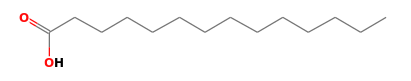
\includegraphics[width=0.7\linewidth]{dados/figuras/Ac_miristico.png}
			\caption[Ácido Mirístico]{Ácido Mirístico  NIST \textit{National Institute of Standards and Technology}}
			\label{fig:nist1}
		\end{figure}
		\item Número do CAS: 544-63-8
		\item Fórmula Molecular: \ch{C14H28O2}
		\item Temperatura de fusão ($T_f$)=327.55 k
		\item Entalpia ($\Delta H_{f}$)=10.771955 kcal/mol
	\end{itemize}
	
	\subsection{Ácido Esteárico}
	\label{sec:2}
	\begin{itemize}
		\item Estrutura
		\begin{figure}[H]
			\centering
			\includegraphics[width=0.7\linewidth]{dados/figuras/Ac_estearico.png}
			\caption[Ácido Esteárico]{Ácido Esteárico NIST \textit{National Institute of Standards and Technology}}
			\label{fig:nist2}
		\end{figure}
		\item Número do CAS: 57-11-4
		\item Fórmula Molecular: \ch{C18H36O2}
		\item Temperatura de fusão ($T_f$)=342.75 k
		\item Entalpia ($\Delta H_{f}$)=14.64126 kcal/mol
	\end{itemize}
	
	\subsection{Ácido Palmítico}
	\label{sec:3}
	\begin{itemize}
		\item Estrutura
		\begin{figure}[H]
			\centering
			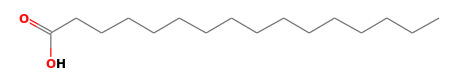
\includegraphics[width=0.65\linewidth]{dados/figuras/Ac_palmitico.png}
			\caption[Ácido Palmítico]{Ácido Palmítico NIST \textit{National Institute of Standards and Technology}}
			\label{fig:nist3}
		\end{figure}
		\item Número do CAS: 57-10-3
		\item Fórmula Molecular: \ch{C16H32O2}
		\item Temperatura de fusão ($T_f$)=336.00 k
		\item Entalpia ($\Delta H_{f}$)=80.252256 kcal/mol
	\end{itemize}
	
	\subsection{1-Hexadecanol}
	\label{sec:4}
	\begin{itemize}
		\item Estrutura
		\begin{figure}[H]
			\centering
			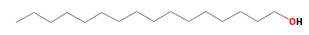
\includegraphics[width=0.8\linewidth]{dados/figuras/Hexadecanol.png}
			\caption[1-Hexadecanol]{1-Hexadecanol NIST \textit{National Institute of Standards and Technology}}
			\label{fig:8}
		\end{figure}
		\item Número do CAS: 36653-82-4
		\item Fórmula Molecular:\ch{C16H34O}
		\item Temperatura de fusão ($T_f$)=322,35k
		\item Entalpia ($\Delta H_{f}$)=8.025226 kcal/mol
	\end{itemize}
	
	\subsection{1-Tetradecanol}
	\label{sec:5}
	\begin{itemize}
		\item Estrutura
		\begin{figure}[H]
			\centering
			\includegraphics[width=0.8\linewidth]{dados/figuras/Tetradecanol.png}
			\caption[1-Tetradecanol]{1-Tetradecanol  NIST \textit{National Institute of Standards and Technology}}
			\label{fig:nist4}
		\end{figure}
		\item Número do CAS: 112-72-1
		\item Fórmula Molecular:\ch{C14H30O}
		\item Temperatura de fusão ($T_f$)=311.00 k
		\item Entalpia ($\Delta H_{f}$)=11.798992 kcal/mol
	\end{itemize}
	
	\subsection{Ácido Linoleico}
	\label{sec:6}
	\begin{itemize}
		\item Estrutura
		\begin{figure}[H]
			\centering
			\includegraphics[width=0.8\linewidth]{dados/figuras/Ac_linoleico.png}
			\caption[Ácido Linoleico]{Ácido Linoleico NIST \textit{National Institute of Standards and Technology}}
			\label{fig:nist5}
		\end{figure}
		\item Número do CAS: 60-33-3
		\item Fórmula Molecular:\ch{C18H32O2}
		\item Temperatura de fusão ($T_f$)=268.15 k
		\item Entalpia ($\Delta H_{f}$)=11.392954 kcal/mol
	\end{itemize}
	